\chapter{Testing}
\section{Overall Approach to Testing}
Testing consisted mainly of manual functional testing due to both a short time scale and visualization of data. As most of the functionality consisted of echoing unit location data to multiple users it was easier the test based on user perception. Some automated tests were created, most notably that of the stress testing of the server instance. 

\section{Client Testing}
\subsection{User Interface Testing}
The Android SDK comes bundled with a number of automated user interface testing tools\footnote{http://developer.android.com/tools/testing/testing\_ui.html}. These functional tests allow for automated testing of component behaviour as well as responding correctly to user actions. This projects interface contained very few components that actually performed very little functionality. One possible candidate for such testing could have been the map views response to using the zoom controls. This however was considered to trivial, along with any other possible test cases, that the time was not invested to automate this process. These functionalities however formed a key role in using the application so would have been quickly picked up by both developer interaction and manual testing.

\subsection{Manual Testing}
Most white-box testing of the client was performed using Androids built in logging methods. LogCat is a greate tool that is bundled with the Eclipse plugin. LogCat allows the tester to view log data in real time from the application running on connected hardware. As well as being an invaluable development tool allowing for real-time debugging errors, it also can be utilised to verify that functions are returning correct values and the application flow is as expected.

Acceptance testing was the most useful testing performed as it validated if the application functioned as intended at the highest level. Each bit of functionality was tested after it's completion and integration into the main application. If a part of the application was not functioning as expected white-boxing techniques were used to pinpoint the location of the problem and rectify it. Even though these tests were only intended to test the new sections of functionality it usual repeating steps from all previous tests to get to that point, thus any problems in previous functionality would be picked up. As well as testing if each section acted as intended it was important to test the application in its entirety. Therefore after each iteration had passed its specific tests a series of steps were carried out intended to cover all currently implemented functionality.

This approach to testing allowed for an increased amount of time spent focused on developing features, however this was possibly at the compromise of the integrity of the application. The use of JUnit to automate the testing of some features would have been a more reliable form of testing. Also investing time in learning and implementing Android specific testing tools, such as UI testing described previously, would have aided this assurance.

\section{Server Testing}
\subsection{Message Generator}
While developing portions of the server program it would have been impractical to use the production client as a primary testing tool. For this reason a small testing suite was created in Python which can be seen in Appendix \ref{server_testing}. This tool creates an easy to use command line interface program that could impersonate the natively running Android client. User input is wrapped in the necessary JSON object and transmitted to the server. Both the sent object and received object are displayed on screen to aid in debugging. 

\begin{figure}[H]
  \centering
   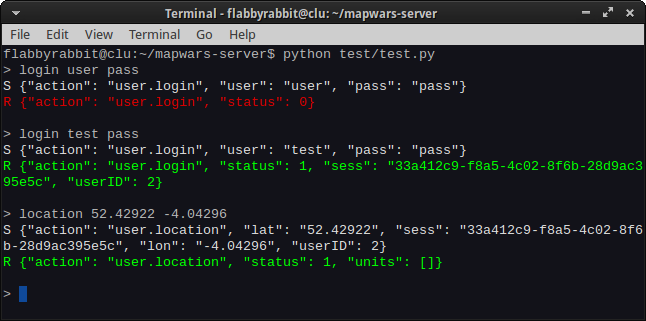
\includegraphics[width=0.8\textwidth]{Images/test.png}
  \caption{The message generator tool in action}
  \label{fig:isogui}
\end{figure}

Although this tool automated the process of generating and transmitting messages it still required the user to decide what is to be sent and to verify what is returned. No logic is presented with the testing tool to decide if the response received is the expected response or not.

\subsection{Stress Testing}
Measuring the stress imposed on the server from increased load was a useful indicator into both the efficiency and stability of code but also the validity of choosing a single server setup. Stress testing was the main automated testing tool with this project. It was a modified version of the message generator tool mentioned previously but removed all user interaction. The program created a connection to the server, registered a user, logged in and set its location. From here it would randomly create and move units at a predetermined fixed interval. By running multiple instances of this program it was possible to simulate any number of connected users performing a heavy load of interactions with the server. To add to this as all units were created within a small area combat between these units was high adding to the stress on the server.

The use of such a test was important to check the efficiency of the server and to try and determine the number of connections each instance could withstand. It was found that memory usage was only effected by unit creation and at a linear rate of 5kb per unit. It was also important to use such a tool to test the clients ability to respond to large volumes of data. While running the stress test against the server the client was also examined running on a mobile device. The minimal increased sluggishness of interactions within the application demonstrated that the client was more than capable of handling large numbers of players in a small area.


\section{User Testing}
To get a feeling for user perception of the application it was given to small focus groups at key stages through out the development process. Feedback was gathered to try and determine their feelings about both game-play and overall experience. Below are two users comments after the final iteration of development.

\renewcommand{\arraystretch}{1.5}
\begin{tabular}{l  p{11cm}}
	\hline
	Name: & Peter Maynard \\
	\hdashline
	Device: & Sony Ericsson ST25i \\
	\hdashline
	Android version: & 2.3.7 Gingerbread \\
	\hdashline
	Screen size: & 3.5 inches, 480 x 854 pixels \\
	\hdashline
	Comments: & Had fun playing around with generating units and fighting them. There was a limited amount of units which was a shame, but can see the potential and look forward to playing with more users. \\
	\hline
\end{tabular}

\begin{tabular}{l  p{11cm}}
	\hline
	Name: & Anika Rusnakova \\
	\hdashline
	Device: & Motorola Xoom 2 ME \\
	\hdashline
	Android version: & 4.0.4 Ice Cream Sandwich \\
	\hdashline
	Screen size: & 8.2 inches, 1280 x 800 pixels \\
	\hdashline
	Comments: & I can see this game becoming very addictive once their are more options and opponents. The map style is perfectly suited to the game as are the simple interface elements. \\
	\hline
\end{tabular}